\section{Polar Codes: Creating Good and Bad Synthetic Channels}

Shannon's theorem proves that reliable codes exist below capacity, but it does not hand us a specific codebook or an efficient decoder. Polar codes address this construction problem with a recursive transformation introduced by Erdal Arıkan. We will first study how the two-bit operator redistributes uncertainty, then place it around actual uses of a binary erasure channel. After applying the operator recursively to four bits, we will generalize the construction, select information and frozen positions, describe the decoder, and state what the polar-coding theorem guarantees.

\subsection{The Two-Bit Transform: An Information-Theoretic Preview}
\label{subsec:polar-core-idea}

A useful way to motivate the transformation is to follow in Arıkan's footsteps and attempt the compression of two bits, which we will call $U$ and $V$. If we keep only their XOR, $(U,V)\to U\oplus V$, the operation is not reversible: several input pairs produce the same output. We therefore keep a second value that is linearly independent of $U\oplus V$, choosing a copy of $V$. The resulting transform is
\begin{equation}
(U,V)\longrightarrow(U\oplus V,V).
\label{eq:polar-transform}
\end{equation}
Given $U\oplus V$ and $V$, we recover $U=(U\oplus V)\oplus V$, so no information is lost. Before placing noisy channels around this operator, we will study how it redistributes uncertainty between two successive tasks: first determining $U\oplus V$, then determining $V$ after the first value is known. This information-theoretic view observes the behavior produced by the polarization operator; the BEC example in the next subsection will connect that behavior to what a receiver can actually decode from noisy outputs.

Although this transformation does not compress the pair, it can redistribute the uncertainty between its two coordinates. To see this in a simple setting, let $U$ and $V$ be independent and identically distributed Bernoulli random variables with
\begin{equation}
\Pr(U=1)=\Pr(V=1)=q,
\qquad 0\leq q\leq\frac12.
\label{eq:polar-bernoulli-inputs}
\end{equation}
The parameter $q$ describes the distribution of these input variables; it is not the BSC crossover probability $p$.
This calculation concerns the uncertainty in the operator's inputs before any noisy outputs are introduced. It is not yet a calculation of a synthetic channel's capacity; choosing $0<q<1/2$ simply makes the operator's redistribution of entropy visible.

\textbf{Statement 1.} For $0<q<1/2$, the probability $q'=\Pr(U\oplus V=1)$ is greater than $q$.

The event $U\oplus V=1$ occurs when exactly one of the two input bits equals $1$. The two possible cases are mutually exclusive, while the random variables $U$ and $V$ are independent. Therefore,
\begin{subequations}
\label{eq:xor-probability-derivation}
\begin{align}
q'
&=\Pr(U\oplus V=1)
\label{eq:xor-probability-definition}\\
&=\Pr(U=1,V=0)+\Pr(U=0,V=1)
\label{eq:xor-probability-cases}\\
&=q(1-q)+(1-q)q
\label{eq:xor-probability-independence}\\
&=2q(1-q).
\label{eq:xor-probability-result}
\end{align}
\end{subequations}
The difference is $q'-q=q(1-2q)$, which is positive for $0<q<1/2$. At the endpoints $q=0$ and $q=1/2$, the difference is zero.

\textbf{Statement 2.} For $0<q<1/2$, the transformation separates the two entropies:
\begin{itemize}
    \item[a)] The first coordinate becomes more uncertain: $H(U\oplus V)>H(U)=H(V)$.
    \item[b)] Once $U\oplus V$ is known, the second coordinate becomes less uncertain: $H(V\mid U\oplus V)<H(U)=H(V)$.
\end{itemize}

Recall that $h_2(q)$ is the entropy of a Bernoulli random variable with parameter $q$. Because $q'>q$ and both values lie between $0$ and $1/2$, $h_2(q')>h_2(q)$. This gives the first inequality.

For the second inequality, we need to compare the uncertainty in the complete pair before and after the transform. The \emph{joint entropy} $H(U,V)$ is the entropy of the pair $(U,V)$ considered as one random object. If $\mathcal{U}$ and $\mathcal{V}$ are the alphabets of $U$ and $V$, and $P_{U,V}(u,v)=\Pr(U=u,V=v)$ is their joint probability, then
\begin{equation}
H(U,V)=-\sum_{u\in\mathcal{U}}\sum_{v\in\mathcal{V}}
P_{U,V}(u,v)\log_2P_{U,V}(u,v).
\label{eq:joint-entropy-definition}
\end{equation}
Because $U$ and $V$ are independent, their joint entropy is the sum of their individual entropies:
\begin{equation}
H(U,V)=H(U)+H(V)=2h_2(q).
\label{eq:independent-joint-entropy}
\end{equation}
The transform is reversible, so the transformed pair contains exactly the same total uncertainty. We now need to separate that total into the uncertainty in the first coordinate and the uncertainty remaining in the second once the first is known. The \emph{chain rule for entropy} states that, for any two discrete random variables $A$ and $B$,
\begin{equation}
H(A,B)=H(A)+H(B\mid A).
\label{eq:entropy-chain-rule}
\end{equation}
Applying this rule to the transformed pair gives
\begin{equation}
H(U\oplus V,V)
=H(U\oplus V)+H(V\mid U\oplus V)
=2h_2(q).
\label{eq:polar-chain-rule}
\end{equation}
Since $H(U\oplus V)=h_2(q')$, we obtain
\begin{equation}
H(V\mid U\oplus V)=2h_2(q)-h_2(q')<h_2(q).
\label{eq:polar-conditional-entropy}
\end{equation}
The first coordinate has therefore become more uncertain, while the second becomes less uncertain once the first is known. From this information-theoretic perspective, the polarization operator has redistributed uncertainty without changing its total amount. Figure~\ref{fig:localpolar} shows the transform.

\begin{figure}[H]
    \centering
    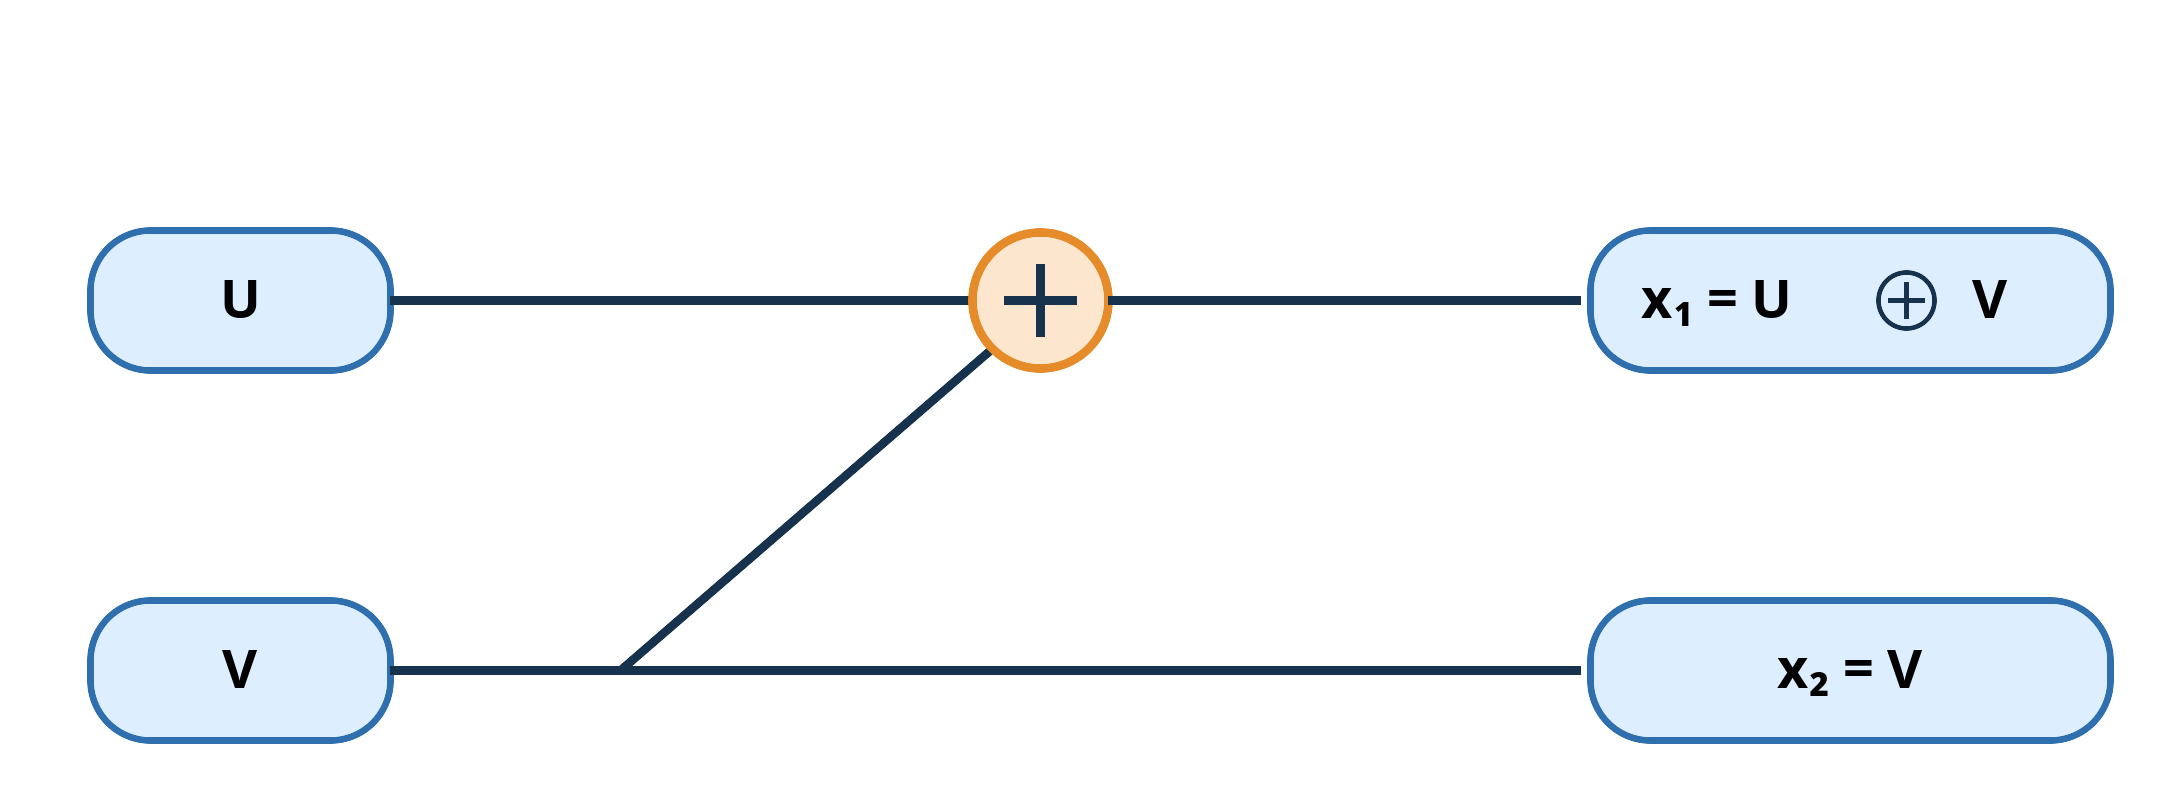
\includegraphics[width=0.88\linewidth]{assets/polar_kernel.png}
    \caption{The reversible transform $(U,V)\to(U\oplus V,V)$. The circled plus denotes XOR.}
    \label{fig:localpolar}
\end{figure}

The entropy calculation gives an information-theoretic preview of the operator: one coordinate becomes more uncertain, the other becomes less uncertain once the first is known, and their total uncertainty is preserved. It does not yet include noisy outputs observed by a receiver. The next subsection places the same transform around two uses of a binary erasure channel, derives the resulting decoding reliabilities, and then applies the calculation recursively to four bits.

\subsection{A Worked Example: The Binary Erasure Channel}

We will now place the transform around actual noisy channel uses. We begin with a two-bit system because one transform is enough to create one less reliable decoding task and one more reliable decoding task. After deriving their reliability formulas, we will apply the same formulas again in a four-bit system to see the recursive effect.

% \begin{samepage}
A \emph{binary erasure channel} with erasure probability $\varepsilon$, written $\operatorname{BEC}(\varepsilon)$, has input $X\in\{0,1\}$ and output $Y\in\{0,1,?\}$. Its behavior is
\begin{equation}
Y=
\begin{cases}
X, & \text{with probability }1-\varepsilon,\\
?, & \text{with probability }\varepsilon.
\end{cases}
\label{eq:bec-definition}
\end{equation}
The channel never changes a $0$ into a $1$ or a $1$ into a $0$. Instead, the symbol ``?'' tells the receiver exactly which positions were erased. We assume that erasures occur independently from one channel use to the next, so the channel is memoryless. An unerased output reveals its input bit completely, while an erased output reveals nothing about that bit. The average information delivered per use, and therefore the capacity, is
\begin{equation}
C_{\mathrm{BEC}}=1-\varepsilon
\qquad\text{bits per channel use}.
\label{eq:bec-capacity}
\end{equation}
% \end{samepage}

\begin{figure}[htbp]
    \centering
    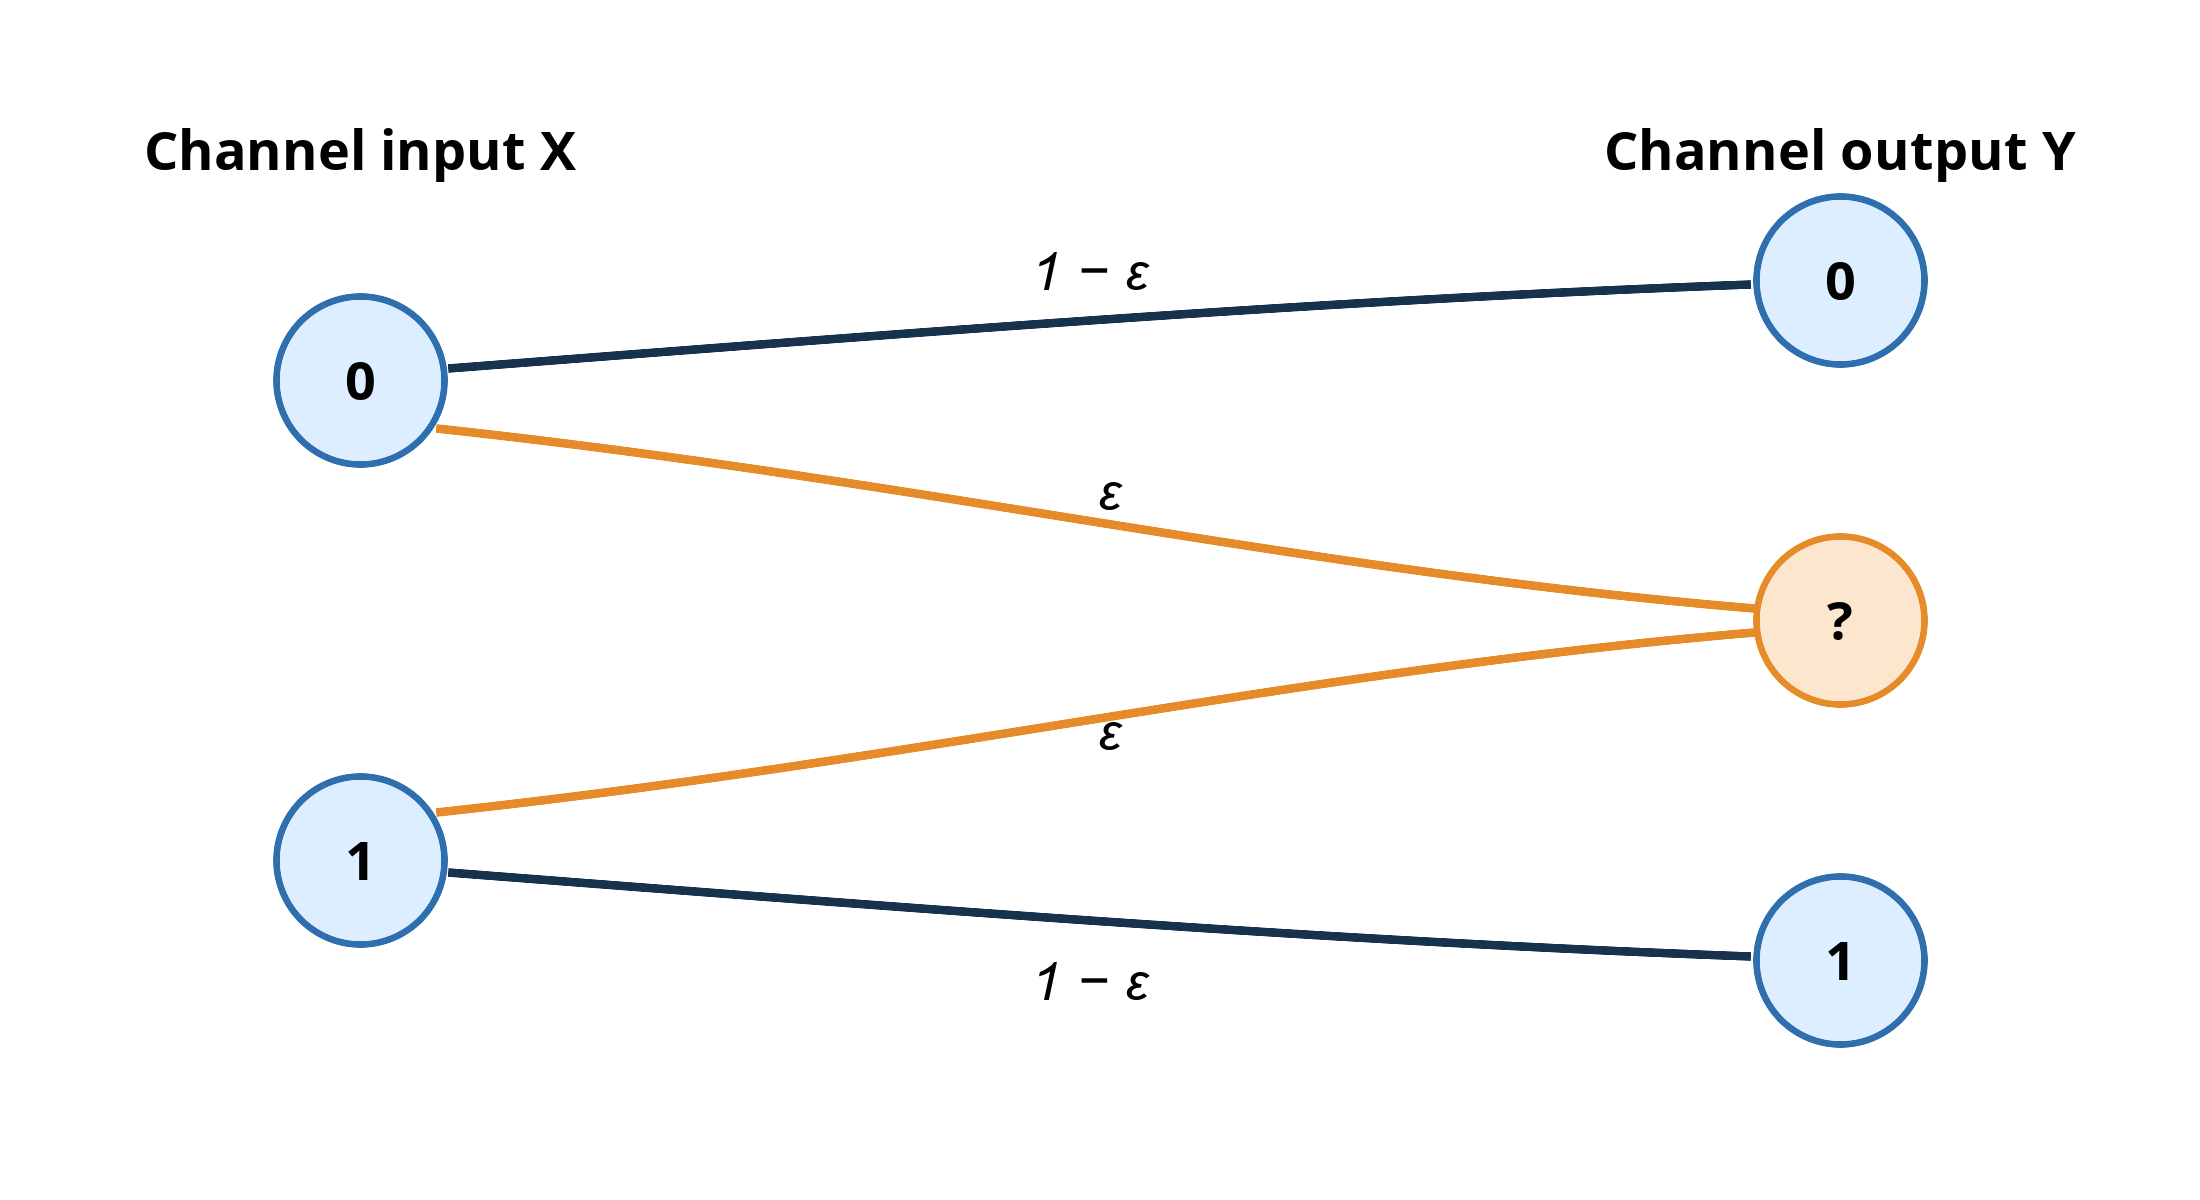
\includegraphics[width=0.78\linewidth]{assets/bec_diagram.png}
    \caption{A $\operatorname{BEC}(\varepsilon)$. The channel delivers the input unchanged with probability $1-\varepsilon$ and outputs the erasure symbol ``?'' with probability $\varepsilon$.}
    \label{fig:bec-transition}
\end{figure}

\subsubsection{The Two-Bit Building Block}

We start with the smallest nontrivial system, which has block length $n=2$. Alice has two independent input bits $u_1$ and $u_2$. For the capacity calculation, each is \emph{equally likely}: independently, each bit equals $0$ with probability $1/2$ and $1$ with probability $1/2$.

The encoder transforms the two inputs into two transmitted bits, and each transmitted bit passes through one independent use of the BEC. The receiver observes $y_1$ and $y_2$ and then estimates the original inputs. The complete two-bit communication chain is
\begin{equation}
\begin{aligned}
(u_1,u_2)
&\xrightarrow{\text{polar encoder}}
(x_1,x_2),\\
(x_1,x_2)
&\xrightarrow{\text{two independent BEC uses}}
(y_1,y_2),\\
(y_1,y_2)
&\xrightarrow{\text{successive decoder}}
(\hat u_1,\hat u_2).
\end{aligned}
\label{eq:bec-two-bit-communication-chain}
\end{equation}
There are two bit positions throughout this system, not six separate information bits. The symbols $u_i$, $x_i$, and $y_i$ describe the input, transmitted value, and observation at each position as it moves through the chain.

First, we encode. Applying Equation~\eqref{eq:polar-transform} gives
\begin{equation}
x_1=u_1\oplus u_2,
\qquad
x_2=u_2.
\label{eq:bec-two-bit-encoding}
\end{equation}
This transform is reversible, so it has not created two additional bits or discarded either input. Alice sends $x_1$ and $x_2$ through the two BEC uses, and each observation $y_i$ is either the corresponding $x_i$ or the erasure symbol ``?''.

Let $W$ denote the original physical channel $\operatorname{BEC}(\varepsilon)$. Combining two independent uses of $W$ with the polar transform creates two \emph{synthetic channels}, meaning two successive decoding tasks built from the same pair of observations. The first, $W^-$, recovers $u_1$ while $u_2$ is unknown. The second, $W^+$, recovers $u_2$ with $u_1$ as side information. The superscripts $-$ and $+$ are branch labels, not arithmetic exponents. A successive decoder actually supplies its earlier estimate $\hat u_1$; the erasure calculation below assumes that estimate is correct. Both tasks use $y_1$ and $y_2$, so neither $x_1$ nor $x_2$ alone corresponds to $W^-$ or $W^+$.

We will now derive a formula for the erasure probability of each task. The two physical BECs entering this transform both have erasure probability $\varepsilon$.

For the minus task, the decoder needs both observations. If $y_1$ and $y_2$ are present, it can compute $u_1=y_1\oplus y_2$. If either observation is erased, one of the required values is missing. The erasure probability is therefore
\begin{subequations}
\label{eq:bec-minus-derivation}
\begin{align}
\varepsilon^-
&=1-\Pr(y_1\neq ?\text{ and }y_2\neq ?)
\label{eq:bec-minus-complement}\\
&=1-(1-\varepsilon)^2
\label{eq:bec-minus-independent}\\
&=2\varepsilon-\varepsilon^2.
\label{eq:bec-minus-result}
\end{align}
\end{subequations}

For the plus task's reliability calculation, $u_1$ is correctly known. The decoder can recover $u_2$ directly from $y_2$, or it can compute $u_2=u_1\oplus y_1$. Thus this synthetic channel is erased only when both observations are erased:
\begin{subequations}
\label{eq:bec-plus-derivation}
\begin{align}
\varepsilon^+
&=\Pr(y_1=?\text{ and }y_2=?)
\label{eq:bec-plus-intersection}\\
&=\varepsilon^2.
\label{eq:bec-plus-result}
\end{align}
\end{subequations}
It is useful to name these two reliability updates
\begin{align}
f(\varepsilon)&=2\varepsilon-\varepsilon^2,
\label{eq:bec-minus-recursion-function}\\
g(\varepsilon)&=\varepsilon^2.
\label{eq:bec-plus-recursion-function}
\end{align}
The function $f$ gives the erasure probability of the minus descendant and $g$ gives that of the plus descendant. Both descendants are themselves BECs of the form shown in Figure~\ref{fig:bec-transition}. We can now verify that their reliabilities have separated:
\begin{subequations}
\label{eq:bec-reliability-separation}
\begin{align}
f(\varepsilon)-\varepsilon&=\varepsilon(1-\varepsilon)>0,
\label{eq:bec-minus-is-worse}\\
\varepsilon-g(\varepsilon)&=\varepsilon(1-\varepsilon)>0,
\label{eq:bec-plus-is-better}
\end{align}
\end{subequations}
for $0<\varepsilon<1$. A larger erasure probability means a less reliable BEC. Equation~\eqref{eq:bec-minus-is-worse} therefore shows that the minus task is less reliable than either original channel, while Equation~\eqref{eq:bec-plus-is-better} shows that the plus task is more reliable. This is the first polarization step.

The capacities of the two synthetic channels are
\begin{align}
C^-(\varepsilon)&=1-f(\varepsilon)=(1-\varepsilon)^2,
\label{eq:bec-minus-capacity}\\
C^+(\varepsilon)&=1-g(\varepsilon)=1-\varepsilon^2.
\label{eq:bec-plus-capacity}
\end{align}
Their sum is
\begin{subequations}
\label{eq:bec-local-capacity-conservation}
\begin{align}
C^-(\varepsilon)+C^+(\varepsilon)
&=(1-\varepsilon)^2+(1-\varepsilon^2)
\label{eq:bec-local-capacity-conservation-expand}\\
&=2(1-\varepsilon),
\label{eq:bec-local-capacity-conservation-result}
\end{align}
\end{subequations}
exactly the combined capacity of the two BECs supplied to the transform. Thus one local transform redistributes reliability without creating capacity.

\subsubsection{Expanding the Construction to Four Bits}

Equations~\eqref{eq:bec-minus-recursion-function} and \eqref{eq:bec-plus-recursion-function} give us a reusable rule: two identical BECs with erasure probability $\varepsilon$ produce descendants with erasure probabilities $f(\varepsilon)$ and $g(\varepsilon)$. This rule makes the analysis recursive. At each new level, $\varepsilon$ denotes the erasure probability entering that particular transform, so we can substitute the previous level's result into the same two functions.

To demonstrate the recursive step, expand to a new block with $n=4=2^2$. This four-bit system has two transform levels. Alice begins with four independent, equally likely inputs $u_1,u_2,u_3,u_4$. The communication chain is
\begin{equation}
\begin{aligned}
(u_1,u_2,u_3,u_4)
&\xrightarrow{\text{polar encoder}}
(x_1,x_2,x_3,x_4),\\
(x_1,x_2,x_3,x_4)
&\xrightarrow{\text{four independent BEC uses}}
(y_1,y_2,y_3,y_4),\\
(y_1,y_2,y_3,y_4)
&\xrightarrow{\text{successive decoder}}
(\hat u_1,\hat u_2,\hat u_3,\hat u_4).
\end{aligned}
\label{eq:bec-four-bit-communication-chain}
\end{equation}
As in the two-bit chain, the different symbols describe the same four positions at different stages.

The encoder first applies the two-bit transform to two pairs of inputs:
\begin{equation}
\begin{aligned}
(v_1,v_2)&=(u_1\oplus u_2,u_2),\\
(v_3,v_4)&=(u_3\oplus u_4,u_4).
\end{aligned}
\label{eq:bec-four-bit-first-encoding-stage}
\end{equation}
It then applies the same transform across the two pairs:
\begin{equation}
\begin{aligned}
(x_1,x_3)&=(v_1\oplus v_3,v_3),\\
(x_2,x_4)&=(v_2\oplus v_4,v_4).
\end{aligned}
\label{eq:bec-four-bit-second-encoding-stage}
\end{equation}
Combining the two stages gives
\begin{equation}
\begin{aligned}
x_1&=u_1\oplus u_2\oplus u_3\oplus u_4,
&x_2&=u_2\oplus u_4,\\
x_3&=u_3\oplus u_4,
&x_4&=u_4.
\end{aligned}
\label{eq:bec-four-bit-encoding}
\end{equation}
Because each local transform is reversible, the complete encoder is also reversible. The four encoded bits then pass through four independent physical BECs.

We now reuse the reliability rule from the two-bit problem. Choose $\varepsilon=1/2$ so that each physical BEC has capacity $1/2$ and the arithmetic remains simple. At the first level of the reliability tree, $f$ and $g$ give the two intermediate erasure probabilities
\begin{align}
f\!\left(\frac12\right)&=\frac34,
\label{eq:bec-four-first-level-minus}\\
g\!\left(\frac12\right)&=\frac14.
\label{eq:bec-four-first-level-plus}
\end{align}
These are the same two reliabilities produced by the two-bit calculation. In the four-bit system, however, they are only intermediate branches. We apply $f$ and $g$ once more to each branch. Table~\ref{tab:bec-four-synthetic-channels} collects the resulting erasure probabilities and capacities. The two branch symbols record the minus or plus choice at each level. Under the input ordering in Equation~\eqref{eq:bec-four-bit-encoding}, $W_4^{(i)}$ is the synthetic channel used to decode $u_i$.

\vspace{0.2cm}

\begin{table}[htbp]
\centering
\begin{tabular}{cclcc}
\toprule
$i$ & Branch & Reliability calculation & Erasure probability $\varepsilon_i$ & Capacity $1-\varepsilon_i$ \\
\midrule
$1$ & $--$ & $f(f(1/2))=f(3/4)$ & $15/16$ & $1/16$ \\
$2$ & $-+$ & $g(f(1/2))=g(3/4)$ & $9/16$ & $7/16$ \\
$3$ & $+-$ & $f(g(1/2))=f(1/4)$ & $7/16$ & $9/16$ \\
$4$ & $++$ & $g(g(1/2))=g(1/4)$ & $1/16$ & $15/16$ \\
\bottomrule
\end{tabular}
\caption{The four synthetic channels obtained from a $\operatorname{BEC}(1/2)$. A smaller erasure probability and a larger capacity both indicate a better synthetic channel.}
\label{tab:bec-four-synthetic-channels}
\end{table}

Their total equals the capacity of the four original BEC uses combined:
\begin{equation}
\frac{1}{16}+\frac{7}{16}+\frac{9}{16}+\frac{15}{16}
=2
=4C_{\mathrm{BEC}}.
\label{eq:bec-four-total-capacity}
\end{equation}
After only two stages, the strongest and weakest synthetic channels are already close to capacities $1$ and $0$. The middle two are less extreme, but further recursion continues the separation. 

\subsection{From Recursion to a Polar Code}
\label{subsec:polar-code-construction}

Consider what happens when we continue applying the same idea recursively. Begin with $n=2^m$ independent uses of the same binary-input channel. At each of the $m=\log_2n$ stages, pair the input coordinates, apply Equation~\eqref{eq:polar-transform}, and repeat the operation across the newly formed groups. The process still produces $n$ synthetic channels; it changes their reliabilities rather than reducing their number. Here, \emph{reliability} describes how likely the input bit of one synthetic channel is to be recovered successfully. It is a property of one synthetic channel, not the block-error probability of the complete code. Block-error probability is the probability that at least one information bit in the decoded block is incorrect. For the binary erasure channels in the worked example above, we measure synthetic-channel reliability by erasure probability: a smaller erasure probability means a more reliable synthetic channel. For other channel models, a different reliability measure may be used. Figure~\ref{fig:polarization} gives a conceptual visualization.

\begin{figure}[H]
    \centering
    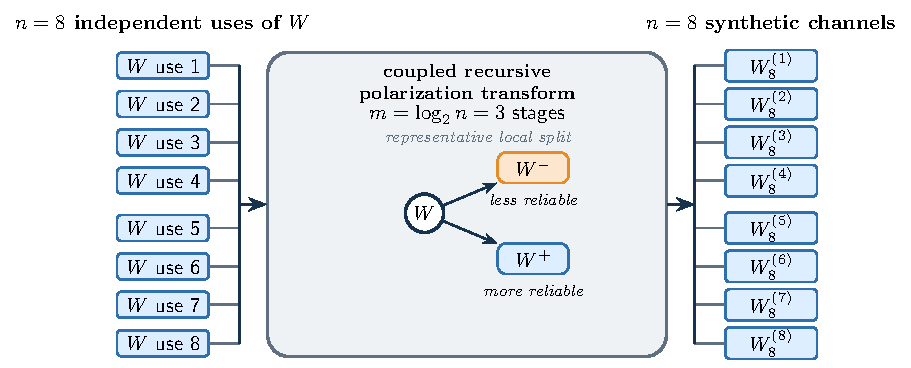
\includegraphics[width=0.95\linewidth]{assets/polarization_recursion.pdf}
    \caption{Conceptual diagram of the recursive polarization process. $n=2^m$ physical channel uses produce $n$ indexed synthetic channels; the indices themselves do not generally rank the channels by reliability.}
    \label{fig:polarization}
    % \par\medskip
    % {\color{red}\small\textbf{Author revision note:} Use $n=8=2^3$ as a concrete example of the general case $n=2^m$. Show the eight independent uses of $W$ entering one coupled, three-stage recursive polarization transform and eight synthetic channels $W_8^{(1)},\ldots,W_8^{(8)}$ emerging. Avoid one-to-one paths between individual physical and synthetic channels. Show $W^-$ and $W^+$ only as representative local less- and more-reliable branches, and make clear that the final channel indices do not rank reliability.\par}
\end{figure}

Thus polar codes use block lengths of the form
\begin{equation}
n=2^m,
\label{eq:polar-block-length}
\end{equation}
where $m=\log_2n$ is the number of recursion stages.

The polarization theorem describes what happens as this process continues. We measure the capacity of each individual synthetic channel by the mutual information $I(U;Y)$ between its input bit $U$ and its output $Y$. Here, $Y$ represents all channel observations and previously decoded input bits made available for that particular decoding task, not merely one physical channel output. We write the capacity of the $i$th synthetic channel as $I(W_n^{(i)})$.

The original physical channel is $W$, and $I(W)$ denotes its \emph{symmetric capacity}: the mutual information obtained when its binary input is equally likely to be $0$ or $1$. As $n$ grows through powers of two, the fraction of synthetic channels with capacity close to $1$ approaches $I(W)$, the fraction with capacity close to $0$ approaches $1-I(W)$, and the fraction with intermediate capacity approaches zero. This statement is asymptotic; at a finite block length, some synthetic channels may still have intermediate reliabilities.

The final result is a set of $n$ synthetic channels with different reliabilities. We use the most reliable channels to send information, while the least reliable channels are \emph{frozen}: their inputs are set to predetermined values known by both the encoder and decoder. We now state this construction rule precisely. For a chosen block length $n$, the transmitter and receiver first rank the synthetic channels according to their reliability. In the BEC example, this is easy because a smaller erasure probability means a more reliable channel. For a general channel, the reliabilities must be calculated or approximated for the chosen physical channel.

Let $\mathcal{A}$ be the set of the $k$ most reliable positions. The input vector $\mathbf{u}=(u_1,\ldots,u_n)$ is filled according to
\begin{equation}
u_i=
\begin{cases}
\text{an information bit}, & i\in\mathcal{A},\\
0\text{, a predetermined frozen bit}, & i\notin\mathcal{A}.
\end{cases}
\label{eq:polar-information-and-frozen-positions}
\end{equation}
Frozen bits may be set to any predetermined values, $0$ or $1$, provided that both the encoder and decoder know them. They do not carry new information, and the decoder does not need to infer them from the noisy output. In this paper, every frozen bit is set to $0$ to simplify the decoder and to keep the resulting polar code linear. Nonzero frozen choices generally produce a translated, or coset, version of the corresponding linear code. The resulting code has rate
\begin{equation}
R=\frac{k}{n}.
\label{eq:polar-code-rate}
\end{equation}

We can now complete the four-bit example rather than stopping at the reliability table. For the $\operatorname{BEC}(1/2)$ in Table~\ref{tab:bec-four-synthetic-channels}, let $n=4$ and $k=2$. The two most reliable positions are $3$ and $4$, so
\begin{equation}
\mathcal{A}=\{3,4\},
\qquad
u_1=u_2=0.
\label{eq:bec-four-information-set}
\end{equation}
If the two message bits are $(a,b)$, they are placed in $(u_3,u_4)$, and Equation~\eqref{eq:bec-four-bit-encoding} gives
\begin{equation}
(a,b)
\longrightarrow
\mathbf{u}=(0,0,a,b)
\longrightarrow
\mathbf{x}=(a\oplus b,b,a\oplus b,b).
\label{eq:bec-four-polar-encoding-example}
\end{equation}
For example, the message $(a,b)=(1,0)$ produces
\begin{equation}
\mathbf{u}=(0,0,1,0),
\qquad
\mathbf{x}=(1,0,1,0).
\label{eq:bec-four-concrete-codeword}
\end{equation}
This example demonstrates how the reliability ranking determines the input placement and how those inputs are encoded. The choice $\mathcal{A}=\{3,4\}$ is specific to the $\operatorname{BEC}(1/2)$ table above; another physical channel may rank the positions differently.

For a block length $n=2^m$, the encoder applies the two-bit XOR transform recursively to the completed vector $\mathbf{u}$. Because the transform uses only XOR and copying, and because all frozen bits are zero, the resulting polar code is a binary linear code of the kind introduced in Subsection 2.5. There are $m=\log_2n$ stages, and each stage performs work proportional to $n$. The total encoding complexity is therefore
\begin{equation}
O(nm)=O(n\log n).
\label{eq:polar-encoding-complexity}
\end{equation}
Big-O notation describes how an operation count grows as the input size increases, rather than giving its exact value. More mathematically, $T(n)=O(n\log n)$ means that there are constants $c$ and $n_0$ such that $T(n)\leq c n\log n$ whenever $n\geq n_0$. Constant factors and smaller-order terms are ignored. The important point is that $n\log n$ grows only slightly faster than $n$, so the encoding remains efficient even for large block lengths.

The qualitative polarization statement explains the achievable rate: if a target rate $R$ is below $I(W)$, then sufficiently large block lengths provide enough channels near capacity $1$ to place information in approximately $Rn$ reliable positions. The stronger claim that the block-error probability also approaches zero requires the rate at which these channels become reliable; that result is included in the polar-coding theorem stated in Subsection~\ref{subsec:polar-theorem}.

\subsection{Successive-Cancellation Decoding}

The previous subsection showed how Alice selects the information positions and encodes the completed input vector. Although the encoder's XOR transformation is reversible, the receiver cannot simply run it backward because the channel outputs may be corrupted or erased. Instead, successive-cancellation decoding uses the channel observations and earlier decisions to recover the input coordinates one at a time. The receiver observes the entire output vector $\mathbf{y}=(y_1,\ldots,y_n)$ and decodes in the forward order
\begin{equation}
u_1,u_2,\ldots,u_n.
\label{eq:successive-cancellation-order}
\end{equation}
This order first appeared in the two-bit example: the receiver estimates $u_1$ through $W^-$ and then uses that decision while estimating $u_2$ through $W^+$. The four-bit construction repeats this dependency recursively. The receiver estimates $u_1$ through $W_4^{(1)}$, then estimates $u_2$ through $W_4^{(2)}$ using the decision about $u_1$, and continues in this way through $u_4$. Thus the synthetic channels are successive decoding tasks built from the same received vector, not isolated physical links.

At a frozen position, the decoder simply inserts the known value $0$. At an information position, it compares how likely $0$ and $1$ are using the entire received vector and all previous decisions, then chooses the more likely value. This method is called \emph{successive-cancellation decoding} because each new decision uses the decisions that came before it. An incorrect early estimate can therefore influence later estimates.

A direct calculation of every conditional probability would repeat a great deal of work. The recursive polar graph allows intermediate likelihood calculations to be reused across decisions. It has $\log_2n$ stages with work proportional to $n$ per stage, giving successive-cancellation decoding complexity
\begin{equation}
O(n\log n).
\label{eq:successive-cancellation-complexity}
\end{equation}
This is the computational benefit of the recursive structure: the encoder and decoder do not need to store or search an arbitrary list of exponentially many codewords.

\subsection{What the Polar-Coding Theorem Does and Does Not Claim}
\label{subsec:polar-theorem}

Polar codes are a family of binary linear codes introduced by Arıkan in 2008. In his complete 2009 journal treatment, he proved that they achieve the symmetric capacity of binary-input memoryless channels while supporting efficient encoding and decoding \cite{Arikan2009}.

We can now state exactly what the construction accomplishes. Arıkan's polarization theorem applies to binary-input discrete memoryless channels and measures rate using the uniform-input mutual information $I(W)$, also called the channel's \emph{symmetric capacity} \cite{Arikan2009}.

\begin{smjtheorem}[Polar coding theorem, simplified]
For a binary-input discrete memoryless channel $W$ and any target rate $R<I(W)$, there exists a family of polar codes with block lengths $n=2^m$ whose rates are at least $R$ and whose block-error probabilities under successive-cancellation decoding approach zero as $n\to\infty$. Encoding and successive-cancellation decoding can be performed in $O(n\log n)$ operations.
\label{thm:polar-coding-simplified}
\end{smjtheorem}

For symmetric channels such as the BSC and BEC, the uniform input distribution is optimal. Their symmetric capacity $I(W)$ therefore equals the ordinary capacity $C$ used in Shannon's theorem. For a nonsymmetric binary-input channel, these two quantities need not be equal, so the theorem above should not automatically be read as a claim that the basic construction reaches the unrestricted capacity of every channel.

Like Shannon's theorem, the polar-coding theorem describes a family as the block length grows. It does not claim that every finite polar code operates at capacity or has zero probability of error. At finite $n$, some synthetic channels remain only partly polarized, their reliabilities must be estimated to select $\mathcal{A}$, and basic successive-cancellation decoding need not give the best practical error performance. The asymptotic achievement is still remarkable: one fixed recursive idea supplies an explicit family whose rate approaches the relevant capacity, whose error probability approaches zero, and whose encoding and decoding complexity grows almost linearly with block length.